\section{Diskussion}
\label{sec:Diskussion}
Abschließend lässt sich feststellen, dass die meisten Messungen sehr präzise sind und nur geringe Fehler aufweisen. Die einziege größere Unsicherheit bei der Messung war das
Stoppen der Fallzeit im Viskosimeter per Stoppuhr. Diese wurde jedoch augenscheinlich durch viele Messungen und Mittelung der Werte gut ausgeschaltet.

Trotz dessen weicht der Wert für die Viskosität von Wasser bei Raumtemperatur um 0,5\% vom Literaturwert ab.


\section{Anhang}
\label{sec:Anhang}

\begin{figure}[H]
    \centering
    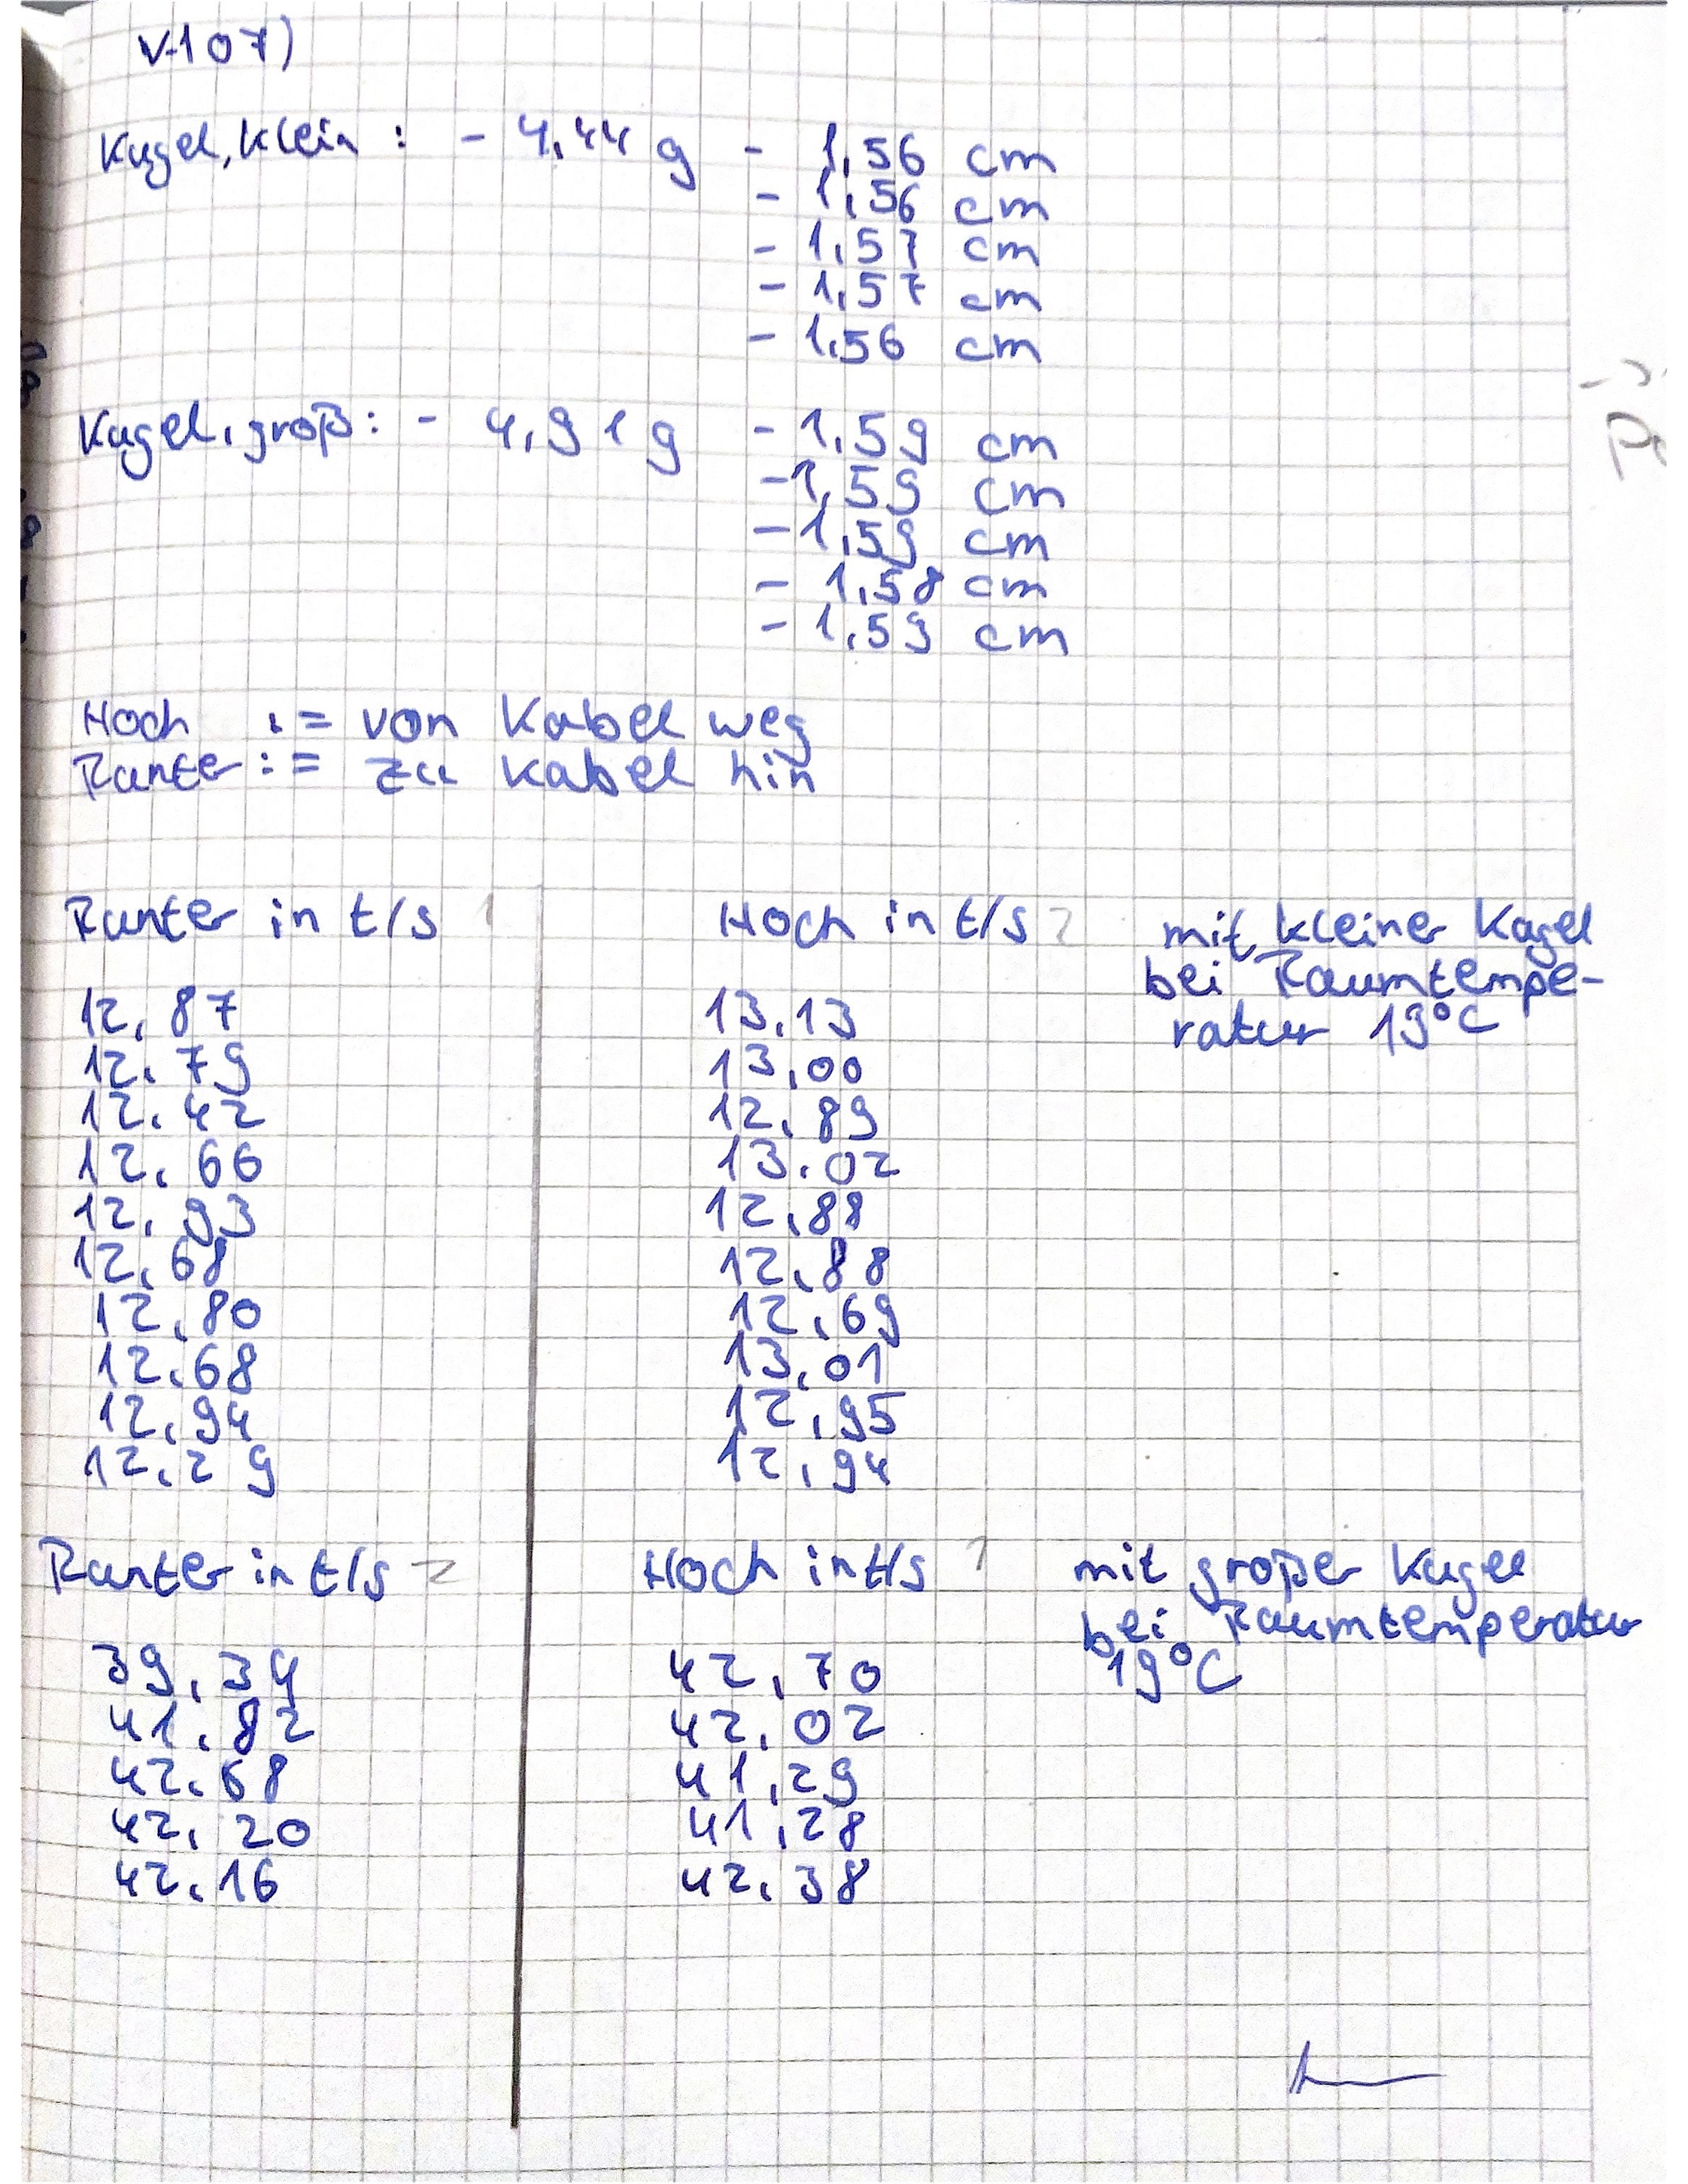
\includegraphics[width=0.5\textwidth]{Dateien/V107daten1.jpg}
    \caption{Originale Messdaten.}
    \label{fig:origDaten1}
\end{figure}
\begin{figure}[H]
    \centering
    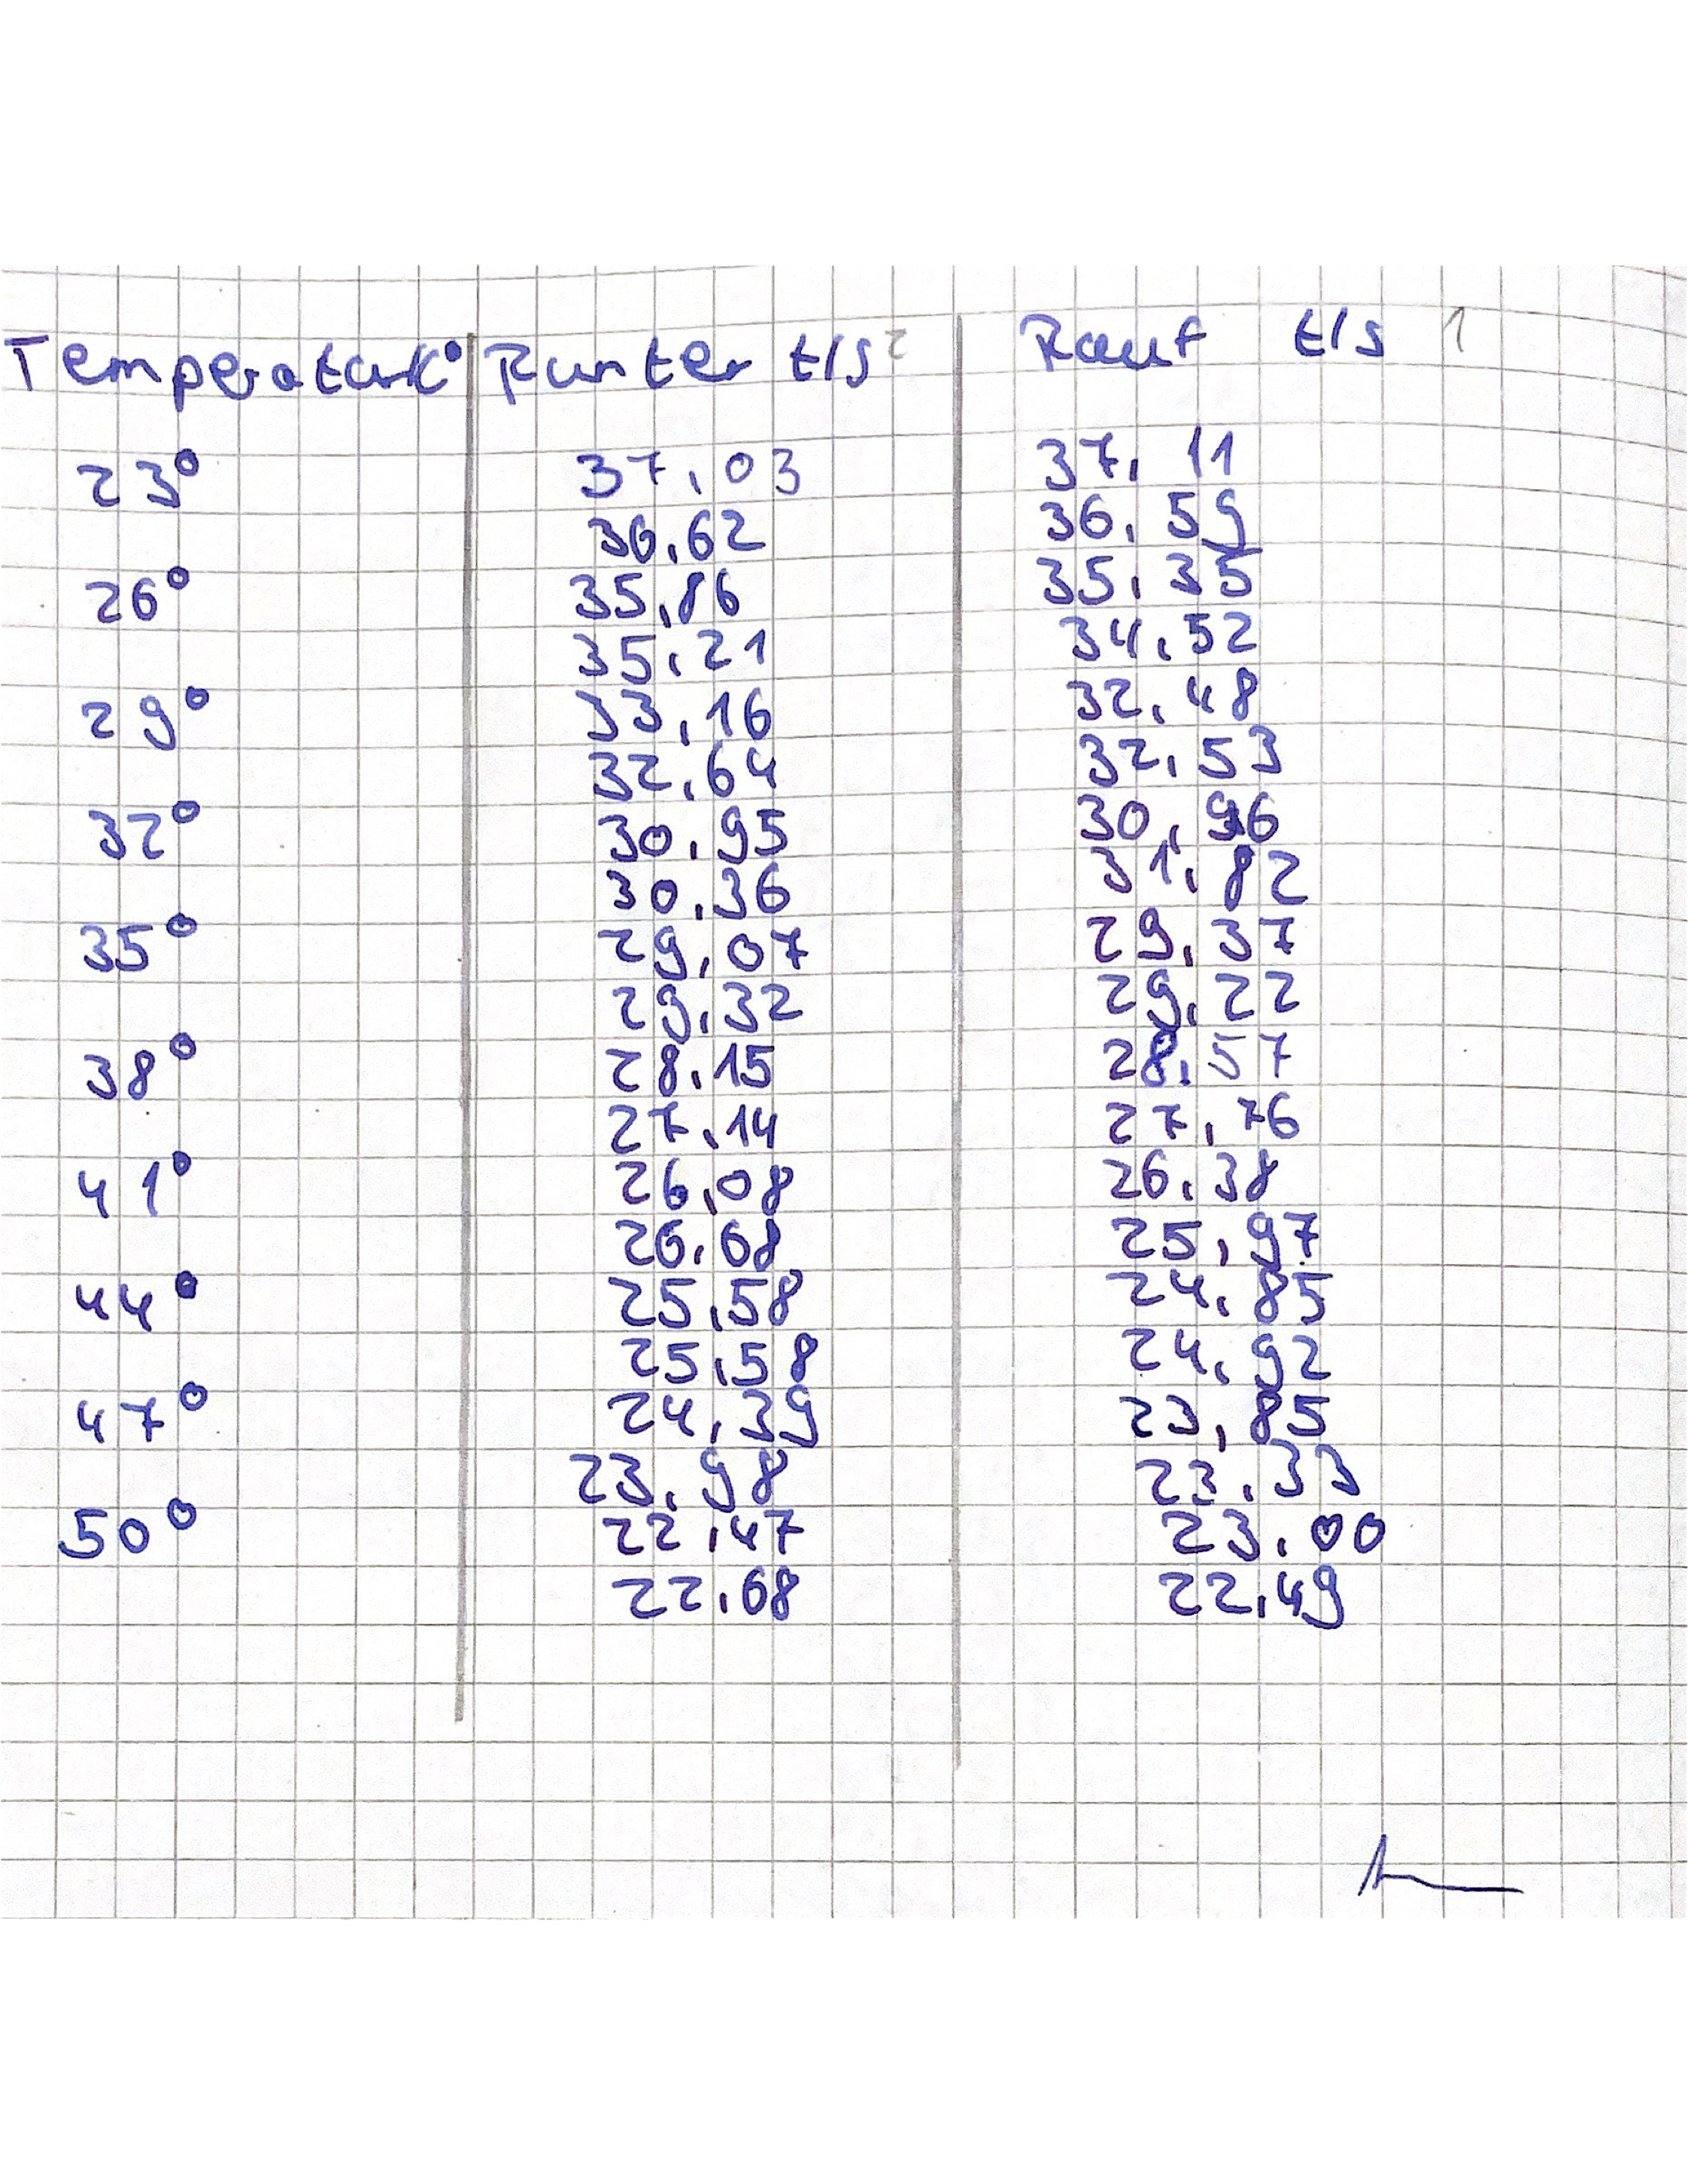
\includegraphics[width=0.5\textwidth]{Dateien/V107daten2.jpg}
    \caption{Originale Messdaten.}
    \label{fig:origDaten2}
\end{figure}